\newcommand{\nom}{Porte conteneur}
\newcommand{\sequence}{03}
\newcommand{\num}{04}
\newcommand{\type}{TD}
\newcommand{\descrip}{Résolution d'un problème en utilisant des méthodes algorithmiques}
\newcommand{\competences}{Alt-C3: Concevoir un algorithme répondant à un problème précisément posé}
\documentclass[10pt,a4paper]{article}
  \usepackage[french]{babel}
  \usepackage[utf8]{inputenc}
  \usepackage[T1]{fontenc}
  \usepackage{xcolor}
  \usepackage[]{graphicx}
  \usepackage{makeidx}
  \usepackage{textcomp}
  \usepackage{amsmath}
  \usepackage{amssymb}
  \usepackage{stmaryrd}
  \usepackage{fancyhdr}
  \usepackage{lettrine}
  \usepackage{calc}
  \usepackage{boxedminipage}
  \usepackage[french,onelanguage, boxruled,linesnumbered]{algorithm2e}
  \usepackage[colorlinks=false,pdftex]{hyperref}
  \usepackage{minted}
  \usepackage{url}
  \usepackage[locale=FR]{siunitx}
  \usepackage{multicol}
  \usepackage{tikz}
  \makeindex

  %\graphicspath{{../Images/}}

%  \renewcommand\listingscaption{Programme}

  %\renewcommand{\thechapter}{\Alph{chapter}}
  \renewcommand{\thesection}{\Roman{section}}
  %\newcommand{\inter}{\vspace{0.5cm}%
  %\noindent }
  %\newcommand{\unite}{\ \textrm}
  \newcommand{\ud}{\mathrm{d}}
  \newcommand{\vect}{\overrightarrow}
  %\newcommand{\ch}{\mathrm{ch}} % cosinus hyperbolique
  %\newcommand{\sh}{\mathrm{sh}} % sinus hyperbolique

  \textwidth 160mm
  \textheight 250mm
  \hoffset=-1.70cm
  \voffset=-1.5cm
  \parindent=0cm

  \pagestyle{fancy}
  \fancyhead[L]{\bfseries {\large PTSI -- Dorian}}
  \fancyhead[C]{\bfseries{{\type} \no \numero}}
  \fancyhead[R]{\bfseries{\large Informatique}}
  \fancyfoot[C]{\thepage}
  \fancyfoot[L]{\footnotesize R. Costadoat, C. Darreye}
  \fancyfoot[R]{\small \today}
  
  \definecolor{bg}{rgb}{0.9,0.9,0.9}
  
  
  % macro Juliette
  
\usepackage{comment}   
\usepackage{amsthm}  
\theoremstyle{definition}
\newtheorem{exercice}{Exercice}
\newtheorem*{rappel}{Rappel}
\newtheorem*{remark}{Remarque}
\newtheorem*{defn}{Définition}
\newtheorem*{ppe}{Propriété}
\newtheorem{solution}{Solution}

\newcounter{num_quest} \setcounter{num_quest}{0}
\newcounter{num_rep} \setcounter{num_rep}{0}
\newcounter{num_cor} \setcounter{num_cor}{0}

\newcommand{\question}[1]{\refstepcounter{num_quest}\par
~\ \\ \parbox[t][][t]{0.15\linewidth}{\textbf{Question \arabic{num_quest}}}\parbox[t][][t]{0.85\linewidth}{#1\label{q\the\value{num_quest}}}\par
~\ \\}

\newcommand{\reponse}[4][1]
{\noindent
\rule{\linewidth}{.5pt}\\
\textbf{Question\ifthenelse{#1>1}{s}{} \multido{}{#1}{%
\refstepcounter{num_rep}\ref{q\the\value{num_rep}} }:} ~\ \\
\ifdef{\public}{#3 ~\ \\ \feuilleDR{#2}}{#4}
}

\newcommand{\cor}
{\refstepcounter{num_cor}
\noindent
\rule{\linewidth}{.5pt}
\textbf{Question \arabic{num_cor}:} \\
}



\begin{document}

\begin{center}
{\Large\bf TP \no {\numero} -- \descrip}
\end{center}

\SetKw{KwFrom}{de} 


\section{Introduction}
\noindent On cherche \` a savoir si deux quantit\' es physiques $X$ et $Y$ sont li\' ees entre elles. Exemple : dans un circuit l'intensit\' e $I$ et la tension $U$.  \\
On dit qu'il y a corr\' elation entre deux variables lorsqu'elles ont tendance \` a varier toujours dans le m\^ eme sens (si $X$ augmente, $Y$ a tendance \` a augmenter) soit toujours dans le sens inverse (si $X$ augmente, $Y$ a tendance \` a diminuer).\\
Pour \' etablir le lien possible entre $X$ et $Y$, on effectue $n$ mesures qui nous donnent $n$ couples $(x_i,y_i)$. \\
Objectif :
\begin{enumerate}
 \item \` a partir de cet \' echantillon, on va quantifier la corr\' elation entre $X$ et $Y$.
 \item si la liaison est lin\' eaire, c'est-\` a-dire si $Y=aX+b$, on va estimer l'\' equation de la droite.
 \end{enumerate} 
Exemple : on a trac\' e le nuage de points pour quatre \' echantillons diff\' erents.\\
Pour quels exemples y'a-t-il liaison entre $X$ et $Y$ ? Et dans ce cas, la liaison est-elle lin\' eaire, non-lin\' eaire ?
\begin{center}
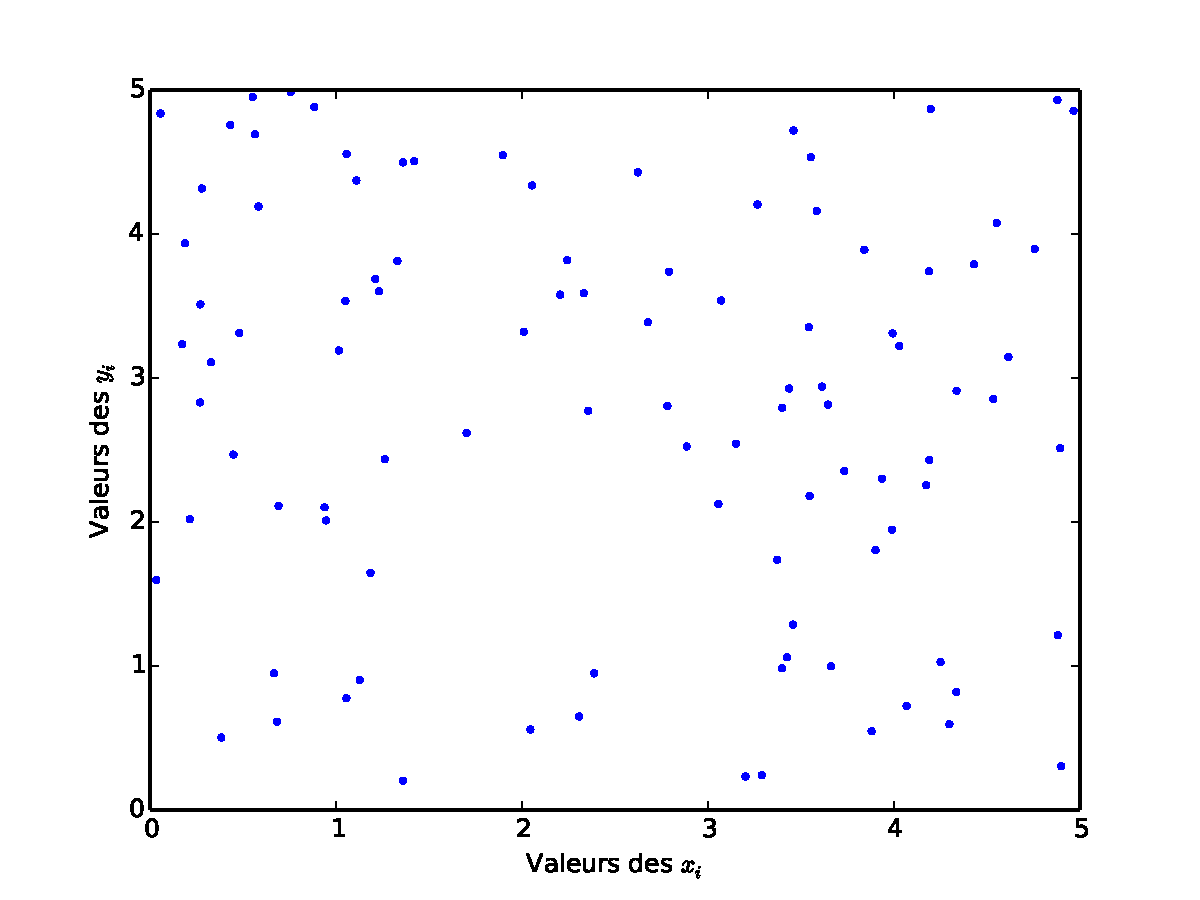
\includegraphics[scale=0.3]{Dessin/Y_Xind.pdf}
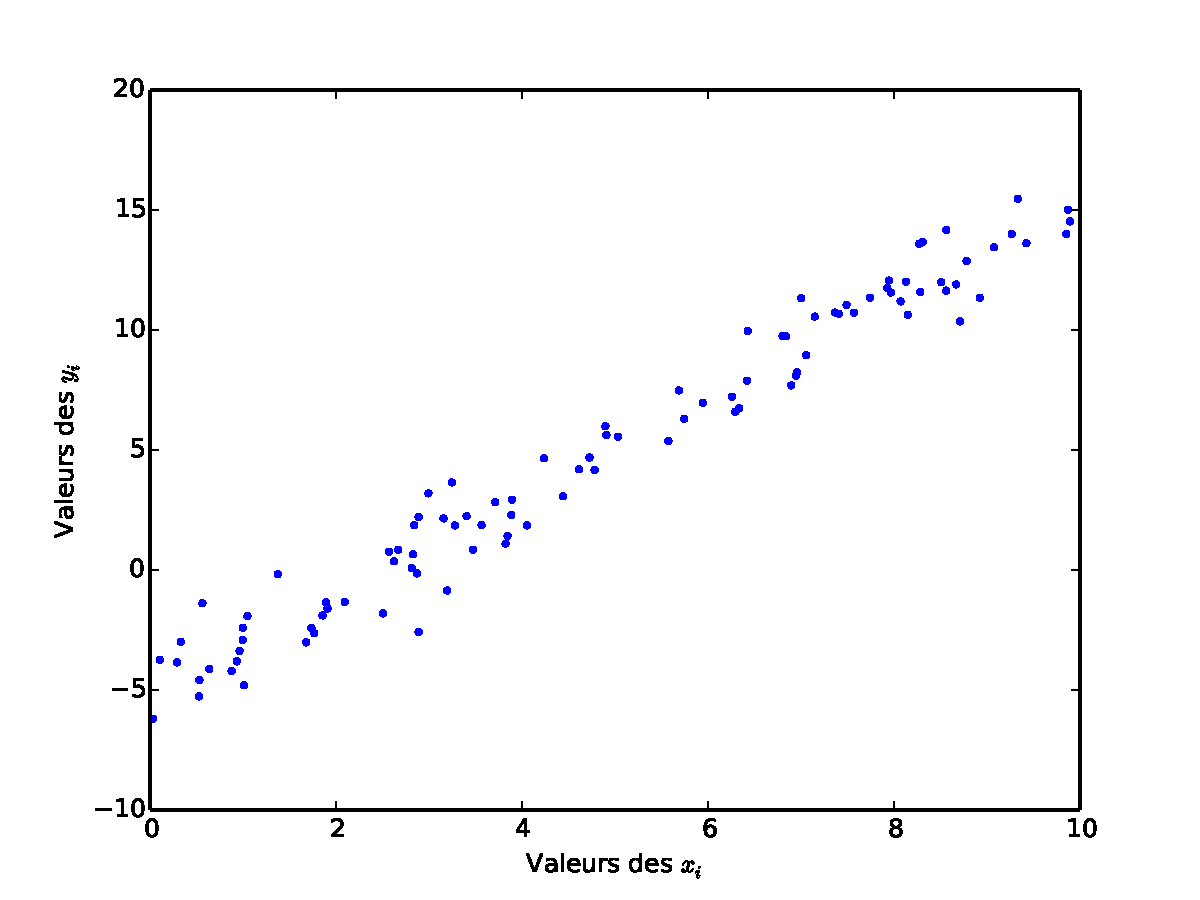
\includegraphics[scale=0.3]{Dessin/XY_lin.pdf}\\
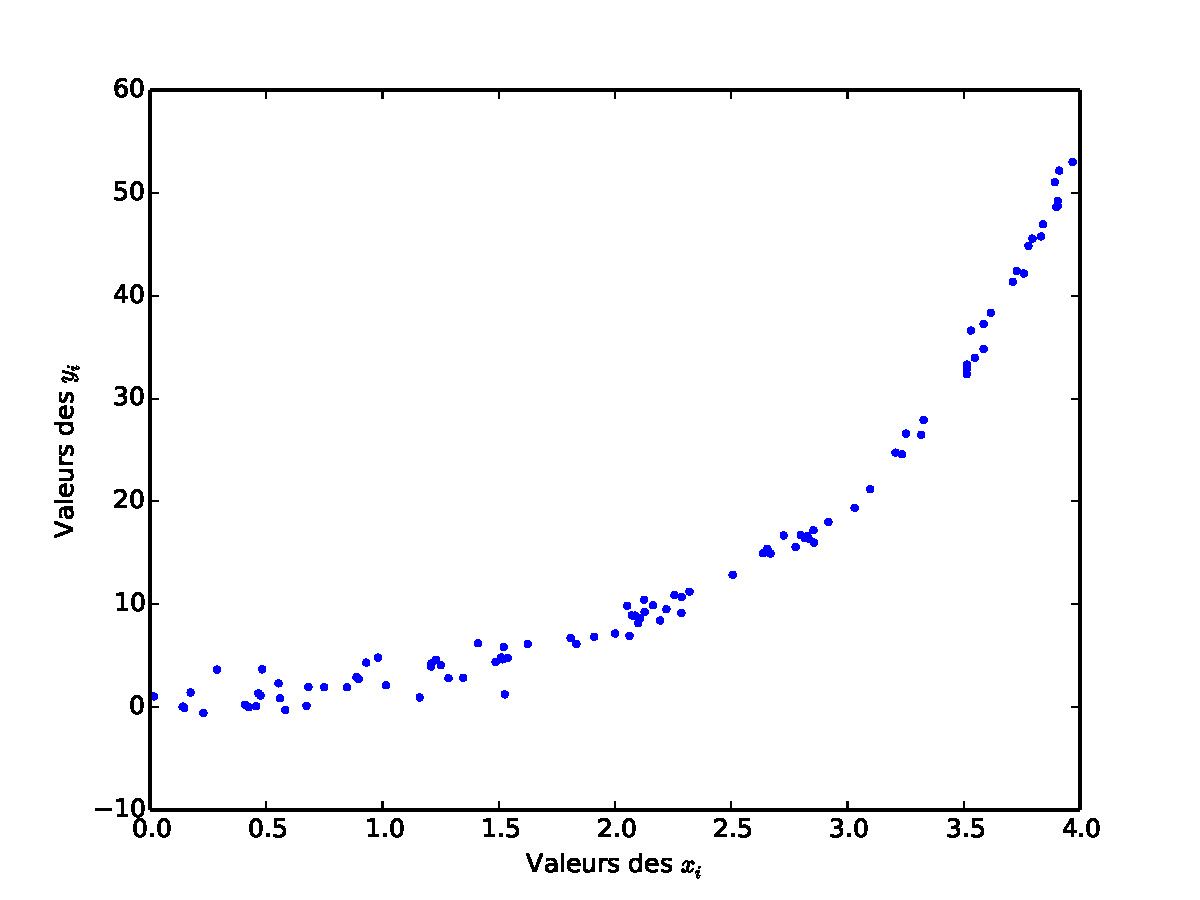
\includegraphics[scale=0.3]{Dessin/Y_expX.pdf}
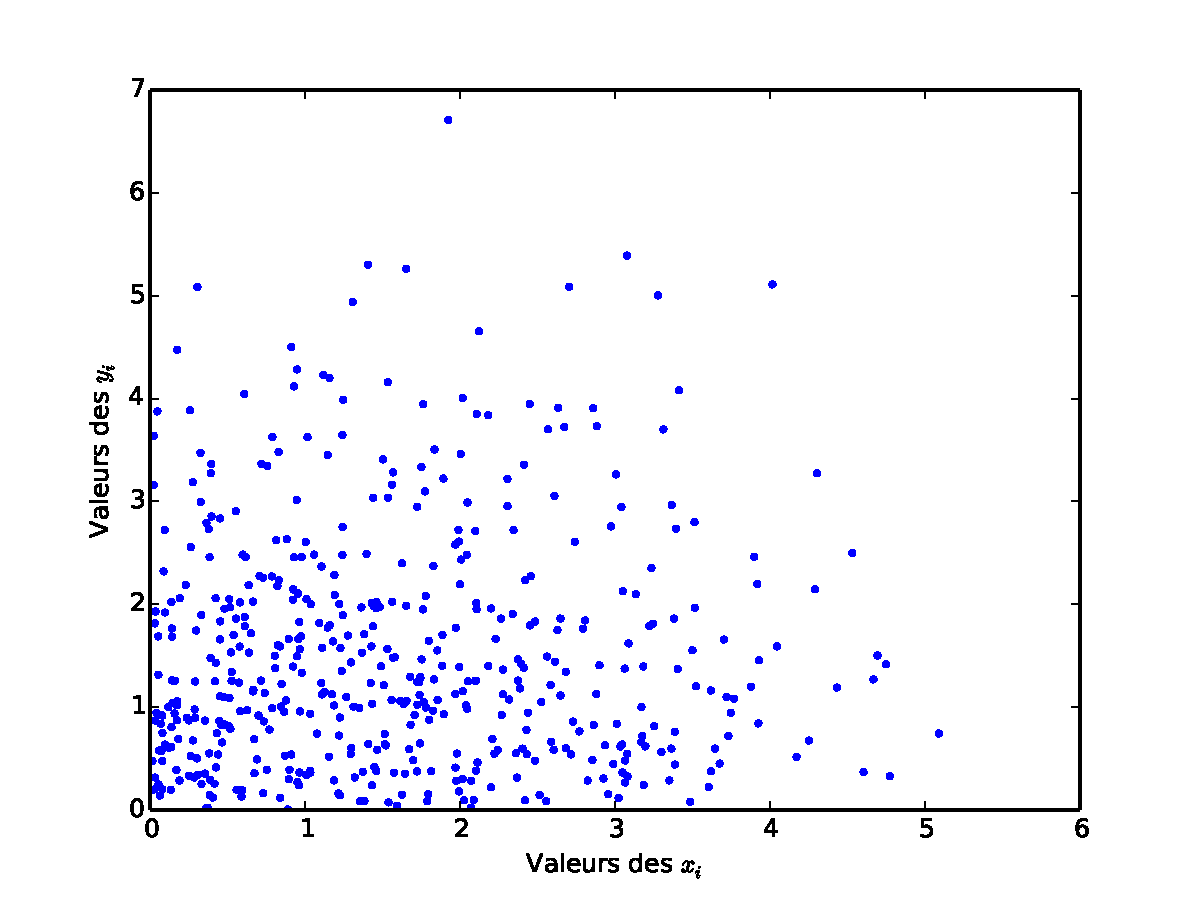
\includegraphics[scale=0.3]{Dessin/Y_Xind2.pdf}
\end{center}
\section{Coefficient de corr\' elation lin\' eaire}
\subsection{La th\' eorie}
\begin{defn}
Soit $X$ et $Y$ deux variables. Le coefficient de corr\' elation lin\' eaire est : 
\[\rho(X,Y)=\dfrac{\mathbb{E}(XY)-\mathbb{E}(X)\mathbb{E}(Y)}{\sigma(X)\sigma(Y)}\hspace*{1cm}\footnote{Pas d'inqui\' etude, nous n'avez pas besoin de savoir ce qu'est $\mathbb{E}(X)$ et $\sigma(X)$ pour faire la suite}\]
\end{defn}

\begin{ppe}
\begin{enumerate}
\item $\rho$ est un nombre compris entre -1 et 1.
\item Il sert \` a quantifier la corr\' elation lin\' eaire entre $X$ et $Y$ :
\begin{enumerate}
\item si $\rho>0$, les variables ont tendance \` a varier dans le m\^ eme sens
\item si $\rho<0$, les variables ont tendance \` a varier dans le sens inverse
\item si $\rho=0$, les variables ne sont pas corr\' el\' ees
\item $\rho=\pm 1$ si et seulement si $Y=aX+b$ (si $\rho =1, a\geqslant 0$, si $\rho=-1, a\leqslant 0$)
\end{enumerate}
\end{enumerate}
\end{ppe}

\noindent Un estimateur de $\rho$ est :\\
\[r=\dfrac{n\displaystyle \sum_{i=0}^{n-1}  x_iy_i-\left(\displaystyle\sum_{i=0}^{n-1}   x_i\right)\left(\displaystyle\sum_{i=0}^{n-1}   y_i\right)}{\sqrt{n\displaystyle\sum_{i=0}^{n-1}   x_i^2-\left(\displaystyle\sum_{i=0}^{n-1}   x_i\right)^2}\sqrt{n\displaystyle\sum_{i=0}^{n-1}   y_i^2-\left(\displaystyle\sum_{i=0}^{n-1}   y_i\right)^2}}\]

\subsection{La pratique}

\begin{exercice}
Soit $X$ une liste de nombres. \' Ecrire une fonction \verb?som? qui renvoie la somme des \' el\' ements de $X$ :
 \begin{minted}[frame=lines]{python}
>>>X=[1,2.1,7]
>>>som(X)
10.1
\end{minted}
\end{exercice}

\begin{exercice}
\begin{enumerate}
\item \' Ecrire une fonction \verb?som_carre? qui renvoie la somme des carr\' es  des \' el\' ements d'une liste.
\item \' Ecrire une fonction \verb?som_prod? qui a comme entr\' ee deux listes de m\^ eme longueur $[x_0,\cdots,x_{n-1}]$ et $[y_0,\cdots,y_{n-1}]$ et renvoie $\displaystyle\sum_{i=0}^{n-1} x_iy_i$.
\item Enfin \' ecrire une fonction \verb?coeff_corr? qui a comme entr\' ee deux listes de m\^ eme longueur $[x_0,\cdots,x_{n-1}]$ et $[y_0,\cdots,y_{n-1}]$ et renvoie l'estimation du coefficient de corr\' elation lin\' eaire $r$. On utilisera les fonctions des questions pr\' ec\' edentes.
\item Que renvoie \verb?coeff_corr(X,X)? ? Pourquoi ?
\end{enumerate}
\end{exercice}


\section{M\' ethode des moindres carr\' es}
\noindent Si le coefficient de corr\' elation lin\' eaire est "assez proche" de 1 ou -1, on cherche la droite qui passe "au plus pr\` es" du nuage de points. Pour \c ca, il faut se fixer un crit\` ere d'ajustement. \\
\begin{minipage}{0.5\textwidth}
On proj\` ete chaque point $(x_i,y_i)$ sur la droite parall\` element \` a $(Oy)$ et on note $\epsilon_i$ l'\' ecart obtenu. 
\end{minipage}
$\quad$
\begin{minipage}{0.9\textwidth}
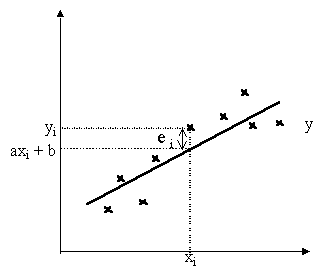
\includegraphics[scale=0.5]{Dessin/projection}
\end{minipage}

\noindent Dans la m\' ethode des moindres carr\' es, on choisit la droite qui minimise la somme des carr\' es des \' ecarts : $\displaystyle\sum_{i=0}^{n-1} \epsilon_i^2$. \\
La droite obtenue est appel\' ee "droite de r\' egression de $Y$ sur $X$".\\
Si la droite de r\' egression s'\' ecrit $y=ax+b$, de "bons" estimateurs de $a$ et $b$ sont :
 \[\hat{a}=\dfrac{n\displaystyle\sum_{i=0}^{n-1}  x_iy_i-\left(\displaystyle\sum_{i=0}^{n-1}   x_i\right)\left(\displaystyle\sum_{i=0}^{n-1}   y_i\right)}{n\displaystyle\sum_{i=0}^{n-1}   x_i^2-\left(\displaystyle\sum_{i=0}^{n-1}   x_i\right)^2}\qquad \hat{b}=\dfrac{\left(\displaystyle\sum_{i=0}^{n-1}  x_i^2\right)\left(\displaystyle\sum_{i=0}^{n-1}  y_i\right)-\left(\displaystyle\sum_{i=0}^{n-1}   x_i\right)\left(\displaystyle\sum_{i=0}^{n-1}   x_i y_i\right)}{n\displaystyle\sum_{i=0}^{n-1}   x_i^2-\left(\displaystyle\sum_{i=0}^{n-1}   x_i\right)^2}\]

\begin{exercice}
\' Ecrire une fonction \verb?dte_reg? qui a comme entr\' ee deux listes de m\^ eme longueur $[x_0,\cdots,x_{n-1}]$ et $[y_0,\cdots,y_{n-1}]$ et renvoie l'estimation de $\hat{a}$ et $\hat{b}$.\\
On utilisera les fonctions pr\' ec\' edentes.\\
Testez la sur $(X,X)$.
\end{exercice}


\begin{exercice}
Application : \\
On a les relev\' es suivants :
\begin{tabular}{|c|cccc|}
\hline
U (V) & 1&2.1&2.9&4\\ \hline
I (mA)&0.99&2.06&3.05&3.98\\\hline
\end{tabular}\\
Les quantit\' es $I$ et $U$ sont-elles corr\' el\' ees ? Si oui, quelle est l'\' equation de la droite de r\' egression lin\' eaire de $U$ sur $I$ ?\\
Que se passe-t-il si on \' echange $I$ et $U$ ? A votre avis, pourquoi ?
\end{exercice}






\ifdef{\public}{\end{document}}{}

\newpage 

\begin{center}
{\Large\bf Correction TP \no {\numero} -- \descrip}
\end{center}



\begin{solution}~\\
\vspace*{-0.7cm}
 \begin{minted}[linenos,frame=lines]{python}
def som(X):
    som=0
    for i in X:
        som=som+i
    return(som)    
\end{minted}
\end{solution}


\begin{solution}~\\
\vspace*{-0.7cm}
\begin{enumerate}
\item 
\begin{minted}[linenos,frame=lines]{python}
def som_carre(X):
    som_carre=0
    for i in X:
        som_carre=som_carre+i**2
    return(float(som_carre)) 
# on renvoie un flottant pour eviter ensuite de diviser par un entier   
\end{minted}
\item  \begin{minted}[linenos,frame=lines]{python}
def som_prod(X,Y):
    som_prod=0
    for i in range(len(X)):
        som_prod=som_prod+X[i]*Y[i]
    return(float(som_prod))  
\end{minted}

\item \begin{minted}[linenos,frame=lines]{python}
def coeff_corr(X,Y):
    n=len(X)
    r=(n*som_prod(X,Y)-som(X)*som(Y))/sqrt(n*som_carre(X)-(som(X))**2)/
    sqrt(n*som_carre(Y)-(som(Y))**2)   
    return(r) 
\end{minted}
\item On trouve \verb?coeff_corr(X,X)=1? car $X$ est \' evidemment fortement corr\' el\' e \` a $X$.
\end{enumerate}
\end{solution}



\begin{solution}~\\
\vspace*{-0.7cm}
 \begin{minted}[linenos,frame=lines]{python}
def dte_reg(X,Y):
    n=float(len(X))
    a=(n*som_prod(X,Y)-som(X)*som(Y))/(n*som_carre(X)-(som(X))**2)
    b=(som_carre(X)*som(Y)-som(X)*som_prod(X,Y))/(n*som_carre(X)-(som(X))**2)
    return(a,b)   
\end{minted}
\verb?dte_reg(X,X)? renvoie \verb?(1,0)? car $X=1\times X+0$.
\end{solution}

\begin{solution}
On trouve un coefficient de corr\' elation lin\' eraire \' egal \` a $\approx 0,99775$ : les variables sont fortement corr\' el\' ees.\\
Les coefficients de la droite de r\' egression lin\' eaire sont $a\approx 1,012$ et $b\approx -0.011$
Si on \' echange $U$ et $I$, le coefficient de corr\' elation n'est pas modifi\' e : le lien entre $X$ et $Y$ est le m\^ eme que celui entre $Y$ et $X$.\\
Par contre, la droite de r\' egression n'est pas la m\^ eme.\\
En effet, dans les formules, $X$ et $Y$ n'ont pas un r\^ ole sym\' etrique. Cela vient du fait qu'on projette parall\` element \` a l'axe $Oy$ sur la droite de r\' egression. \\
On a plusieurs choix pour la droite qui passe au plus pr\` es du nuage de points. Dans la m\' ethode des moindres carr\' es pr\' esent\' ee ici, $X$ est dite la variable pr\' edictive ou explicative et $Y$ la variable \` a expliquer.
\end{solution}

\end{document}












